\section{Theorie}
\label{sec:Theorie}
Das Ziel dieses Versuches ist es, die Elastizitätsmodule verschiedener Materialien zu ermitteln und die erhaltenen Werte mit den Literaturwerten zu vergleichen.
\\
Die physikalische Größe der mechanischen Spannung $\sigma_\text{m}$ ist definiert durch die wirkende Kraft $F$ auf eine Fläche $A$.
Eine auf einen Körper wirkende Spannung kann eine Gestalts- und Volumenveränderung hervorrufen.
Unterteilt wird diese Größe in die senkrecht zur Oberfläche stehende Komponente, der sogenannten Normalspannung $\sigma$ und die zur Oberfläche parallele Komponente, der sogenannten Tagential oder Schubspannung.
wirkt durch Druck oder Zug eine Spannung in nur eine Körperdimension vor, so ist diese Proportional zur Längenänderung $\sfrac{\symup{\Delta}L}{L}$ und es folgt das Hooksche Gesetz
\begin{equation}
    \sigma=E \frac{\symup{\Delta}L}{L}
\end{equation}
mit dem materialspezifischen Elastizitätsmodul $E$ als Proportionalitätsfaktor. 
Mit Hilfe einer hinreichend genauen Messvorrichtung könnte das Elastizitätsmodul aus kleinen Längenänderungen $\symup{\Delta}L$ eines stabförmigen Körpers bestimmt werden.
In diesem Versuch wird jedoch mit Hilfe der Biegung, die bereits bei relativ geringen Kräften eine leicht messbare Veränderung am Probenstab hervorruft, der Elastizitätsmodul bestimmt.
Dabei werden zwei unterschiedliche Arten der Biegung untersucht. Diese sind in Abbildung \ref{fig:drei} dargestellt und unterscheiden sich in der Einspannung und der Positionierung des Gewichtes.
\begin{figure}
    \begin{subfigure}{0.48\textwidth}
        \centering
        \caption{Biegung eines einseitig eingespannten elastischen Stabes}
        \label{fig:eins}
        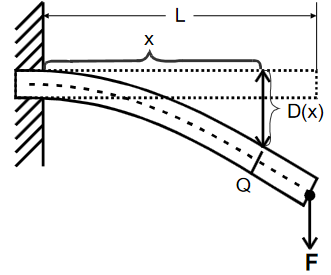
\includegraphics[height=4.5cm]{pics/eins.png}
    \end{subfigure}
    \begin{subfigure}{0.48\textwidth}
        \centering
        \caption{Biegung eines zweiseitig aufgelegten Stabes}
        \label{fig:zwei}
        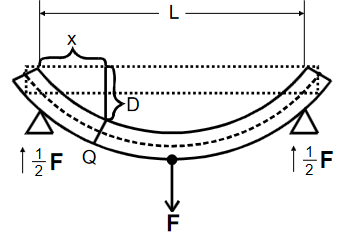
\includegraphics[height=4.5cm]{pics/zwei.png}
    \end{subfigure}
    \caption{Biegung mit beid- und einseitiger Einspannung.
    Die gestrichelte Linie markiert die neutrale Faser, die ihre Länge beibehält.}
    \label{fig:drei}
\end{figure}
Die dabei gemessene Messgröße $D$ ist bei sonst gleichen Verhältnissen der Kraft und der Abmessungen des Stabes sehr viel größer als $\symup{\Delta}L$.
\subsection{Durchbiegung eines homogenen Stabes einseitiger Einspannung}
Bei der einseitigen Einspannung sind die Längenänderungen nicht mehr konstant. Daher muss die Durchbiegung $D(x)$ als Funktion des Ortes errechnet werden.
Da in der Funktion $D(x)$ der Elastizitätsmodul auftaucht, kann die Materialkonstante mit Hilfe einer Messreihe der Größen $D$ und $x$ bestimmt werden.
Die am uneingespannten Ende des Stabes wirkende Gravitationskraft $F$ eines aufgehängten Gewichtes bewirkt ein angreifendes Drehmoment
\begin{equation}
    M_\text{F}=F \left(L-x\right)
\end{equation}
mit der Länge des Hebelarms $\left(L-x\right)$. Es kommt zu einer Dehnung der oberen und eine Stauchung der unteren Stabschichten, sodass sich der Querschnitt in verdrehter Position befindet.
Dabei behält die neutrale Faser in der Mitte des Querschnitts $Q$ seine Länge bei. Die Zug- und Druckspannungen, die an $Q$ angreifen sind entgegengesetzt gleich und bewirken so ein Drehmoment $M_\sigma$, welches sich
durch Integration über $Q$ mit 
\begin{equation}
    M_\sigma=\int_\text{Q} y\sigma (y) \symup{d}q
\end{equation}
berechnen lässt, worin $y$ den Abstand des Flächenelementes $\symup{d}q$ von der neutralen Faser $x$ bedeutet. Daraus lässt sich für die Durchbiegung die Formel
\begin{equation}
    D(x)=\frac{F}{2 E I}\left(L x^2 - \frac{x^3}{3}\right)  \qquad (\text{für} \, 0 \leq x \leq L)
    \label{eqn:deins}
\end{equation}
herleiten mit dem Flächenträgheitsmoment
\begin{equation}
    I=\int_\text{Q} y^2 \symup{d}q(y) \, .
    \label{eqn:fltm}
\end{equation}
\subsection{Durchbiegung eines Stabes zweiseitiger Auflage}
An den Auflagestellen des beidseitig aufgelegten Stabs wirkt nach Abbildung \ref{fig:zwei} die Gravitationskraft $\sfrac{F}{2}$ des Gewichtes in der Mitte der Querschnittsfläche mit einem 
Hebelarm der Länge $x$. Dadurch wirken die Drehmomente
\begin{align}
    M_\text{F}& = - \frac{F}{2} x   & \left(\text{für}\,\, 0 \leq x \leq \frac{L}{2}\right) \\
    M_\text{F}& =-\frac{F}{2}(L-x)  & \left(\text{für}\, \,\frac{L}{2} \leq x \leq L \right)
\end{align}
woraus sich die Durchbiegung
\begin{align}
    D(x)&= \frac{F}{48 E I} \left(3 L^2 x - 4 x^3 \right) & \left(\text{für}\,\, 0 \leq x \leq \frac{L}{2}\right) \\
    D(x)&= \frac{F}{48 E I} \left(4x^3 -12 L x^2 + 9 L^2 x - L^3\right) & \left(\text{für}\, \,\frac{L}{2} \leq x \leq L \right)
\end{align}
ergibt.